\chapter{Supplemental material for \chapref{chap:neocortex}}
\label{chap:neocortexSuppl}

\begin{figure}[htbp]
\centering
\begin{tabular}{l}
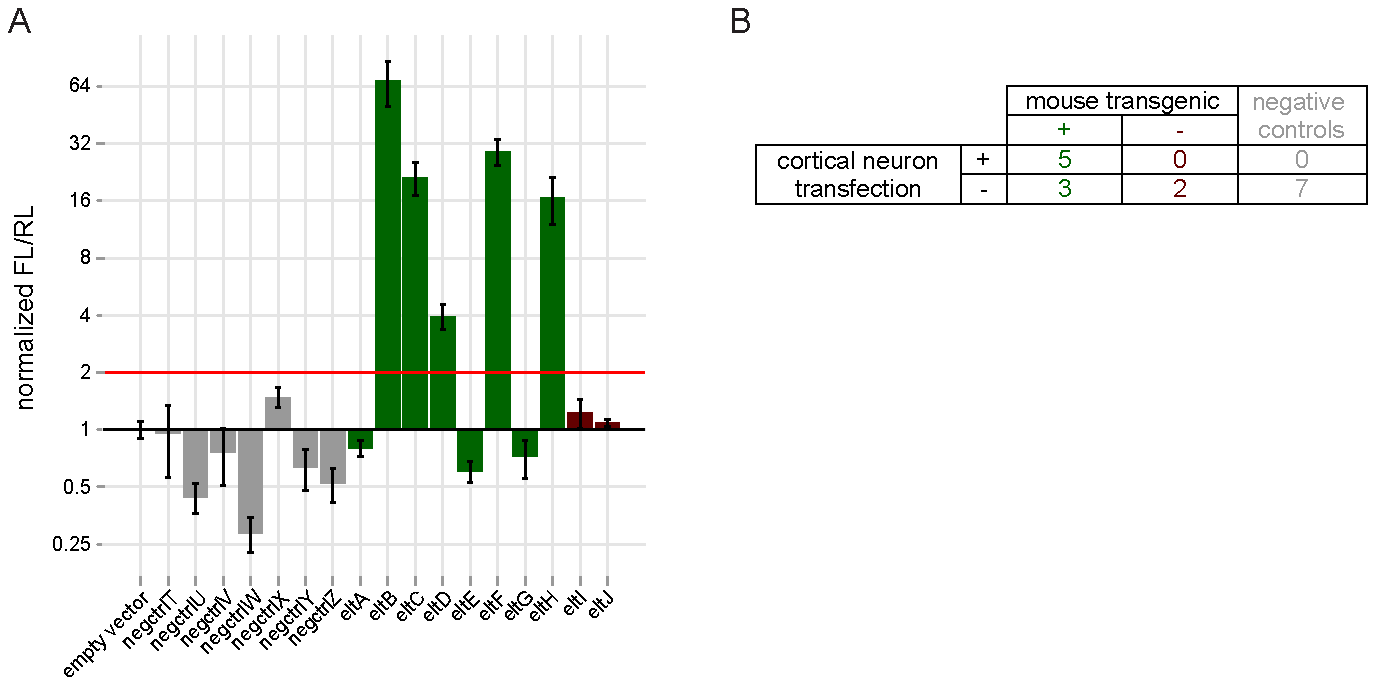
\epsfig{file=figures/ncxFigureS1.pdf,width=0.99\linewidth,clip=,trim=0 0 0 0} \\
\end{tabular}
\caption[\textit{In vitro} transfection of dissociated cortical neurons approximates \textit{in vivo} enhancer activity] {
{\bf \textit{In vitro} transfection of dissociated cortical neurons approximates \textit{in vivo} enhancer activity.}
{\bf (A)} Enhancer activity in dissociated E14.5 cortical neurons.  gray: negative control elements randomly selected
from the genome; green: positive \textit{in vivo}; red: negative \textit{in vivo}; black line: 2 fold empty vector,
the cutoff to call a positive enhancer element
{\bf (B)} Agreement between \textit{in vivo} mouse transgenic enhancer assay and \textit{in vitro} cortical neuron
transfection assay.  All elements that function as enhancers \textit{in vitro} also are positive \textit{in vivo}.
}
\label{fig:ncxFigS1}
\end{figure}

\begin{table}[htbp]
\label{tab:ncxTableS1}
\begin{center}
{
\begin{tabular}{c|l}
Element & Genomic Coordinates (mm9)\\
\hline
eltA & chr9:118,236,674-118,237,901\\
eltB & chr1:57,386,010-57,387,590\\
eltC & chr11:98,144,466-98,146,103\\
eltD & chr2:61,588,525-61,590,055\\
eltE & chr5:132,277,438-132,278,862\\
eltF & chr13:47,508,530-47,509,889\\
eltG & chr3:18,643,303-18,644,789\\
eltH & chr5:132,504,807-132,506,235\\
eltI & chr6:143,387,503-143,388,486\\
eltJ & chr12:108,454,032-108,454,724\\
negctrlT & chr18:76,976,654-76,977,772\\
negctrlU & chr11:15,019,789-15,021,400\\
negctrlV & chr4:142,134,795-142,136,312\\
negctrlW & chr11:63,723,196-63,724,604\\
negctrlX & chr10:21,516,932-21,518,391\\
negctrlY & chr14:76,694,740-76,696,003\\
negctrlZ & chr15:95,074,004-95,075,437\\
\end{tabular}
}
\caption[Selected enhancer candidates] {
{\bf Selected enhancer candidates.}
Genomic coordinates (mm9) of the neocortex p300 peaks selected to test for enhancer activity.
}
\end{center}
\end{table}
